\subsection{Organisation des SVN-Repositories}

Die \marginpar{Ordnerstruktur} Strukturierung der Ordner ist wohl das wesentliche Hauptmerkmal des SVN. SVN arbeitet mit der Idee der Kopie. Das bedeutet, man besitzt eine Hauptentwicklungslinie die den Stamm des kompletten Projektes bildet. Im Falle des Studienprojektes \glqq DecidR\grqq{} (vgl. Abbildung \ref{fig:ordner}) ist \texttt{trunk} der Hauptordner, indem das Hauptprojekt abgespeichert wird. Da es dabei sinnlos ist, alle Dateien nur in dem \texttt{trunk} Ordner zu legen, ist eine weitere Untergliederung sinnvoll. Es wurden die Ordner \texttt{docs}, \texttt{prototype}, \texttt{seminars} und \texttt{src} angelegt. 

Im Unterordner \texttt{docs} befinden sich alle Dokumente, die in diesem Projekt erstellt werden (Angebot, Anforderungsanalyse, Spezifikation, Entwurf, Test, Handbuch usw.). F�r jedes weitere Dokument wurde ein weiterer Unterordner angelegt, indem dann die kompletten Dateien abgelegt werden. 

Der Unterordner \texttt{prototype} dient zur Ablage der Dateien f�r den Prototypen. Auch dieser enth�lt Unterordner, die sich speziell auf das Subprojekt beziehen. 

Der Ordner \texttt{seminars} bietet den Teammitgliedern die M�glichkeit ihr eigenes Seminar per Versionskontrolle zu erstellen. Jedes Teammitglied besitzt einen eigenen Ordner, den er selber weiter gestalten kann, wie er m�chte. 

Und im Unterordner \texttt{src} wird der Hauptcode abgelegt, der w�hrend der Implementierungsphase ensteht. 

Zudem gibt es noch den Ordner \texttt{tags}. Dieser Ordner dient der Markierung von gewissen Versionsst�nden. Hier werden alle Versionen abgelegt, die als stabil erachtet werden oder als Review-Version dienen. Das bedeutet, falls der erste Prototyp lauff�hig ist, wird die Version dort abgelegt, damit die Entwickler zu einem sp�teren Zeitpunkt genau wissen, auf welche Version sie sich berufen m�ssen, falls sie etwas am fertigen Prototypen �ndern m�chten. 

Letztlich bleibt noch der Ordner \texttt{branch}. In diesem Ordner werden nach der Philosophie des SVN Kopien des Stammordners \texttt{trunk} angelegt, um, wenn evtl. n�tig, andere Entwicklungspfade einzuschlagen. Der Ordner ist somit ein Zweig der Hauptentwicklungslinie. Man kann dann andere Entwicklungpfade einschlagen, ohne die Hauptentwicklungslinie zu besch�digen. 

\begin{figure}[h]
 \centering
 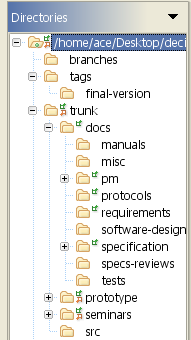
\includegraphics[scale=0.6]{ordertree.png}
 \caption{Ordnerstrukur des Studienprojektes \glqq DecidR\grqq{}}
  \label{fig:ordner}
\end{figure}

Diese Ordnerstruktur wird als Standard angesehen und von allen SVN Betreibern empfohlen. Letzten Endes bleibt es dem Versionsbeauftragtem �berlassen, wie er das SVN strukturiert. Der Versionsbeauftragte ist die Person im Projekt, die sich um die Ordnerstruktur im SVN k�mmert.
